\documentclass{article}
\usepackage{graphicx}  
\usepackage{subfigure}  

\begin{document}

\title{Side-by-Side Figures Example}
\author{Nihar Debnath \\ Roll Number: 30001223008 \\ Department: Bachelors of Computer Application}
\date{\today}
\maketitle

\begin{figure}[htbp]
    \centering
    \subfigure[MAKAUT LOGO]{
        
\includegraphics[width=0.45\textwidth]{image1.jpg}  % Replace with your image file
        \label{fig:first}
    }
    \hfill
    \subfigure[MAKAUT ORIGIBNAL PICTURE]{
        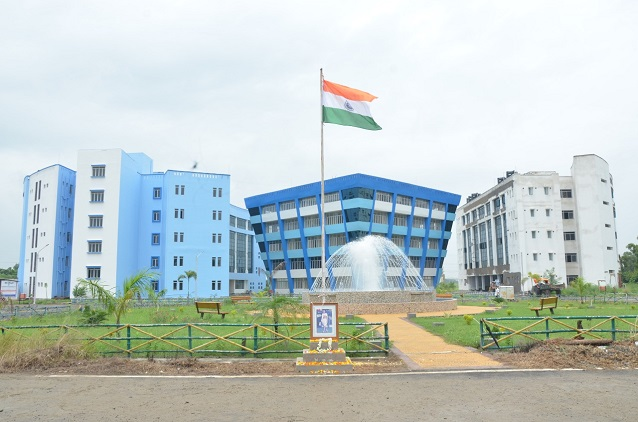
\includegraphics[width=0.45\textwidth]{image2.jpeg}  % Replace with your image file
        \label{fig:second}
    }
    \caption{MAKAUT PICTURES}
    \label{fig:sidebyside}
\end{figure}

\section{Introduction}
This document shows how to create side-by-side figures using the \texttt{subfigure} package in LaTeX. 

\end{document}

